\subsection{循环队列}

\begin{frame}\ft{\subsecname}
\begin{figure}
  \centering
  \begin{tikzpicture}
    \tikzstyle{information text}=[rounded corners,fill=blue!10,inner sep=1ex]
    \def\x{0.75}
    \def\y{0.75}

    \foreach \c in {0}{
      \ifthenelse{\c=0}{
        \def\r{0}
        \draw[very thick](\r*\x,\c*\y)--(\r*\x+5*\x,\c*\y);
        \draw[very thick](\r*\x,\c*\y+\y)--(\r*\x+5*\x,\c*\y+\y);        
        \foreach \r in {0,1,2,3,4}{                   
          \node[]at(\r*\x+0.5*\x,\c*\y-0.5*\y){\small $\r$};
        }

        \foreach \r in {1,2,3,4,5}{         
          \draw[](\r*\x-\x,\c*\y+0.1*\y)rectangle(\r*\x-0.1*\x,\c*\y+0.9*\y);
        }
        \foreach \r in {1,2,3}{         
          \node[]at(\r*\x-0.5*\x,\c*\y+0.5*\y){$a_{\r}$};
        }
        \def\r{3}
        \draw[<-,very thick](\r*\x-0.3*\x,\c*\y+0.7*\y)--(\r*\x-0.2*\x,\c*\y+1.5*\y) node[above]{ 队尾};

        \pause
        \def\rr{8}
        \draw[very thick,->](\rr*\x-2.8*\x,\c*\y+0.5*\y)--node[above]{入队列}(\rr*\x-0.2*\x,\c*\y+0.5*\y);
        \pause
        
        \draw[very thick](\rr*\x,\c*\y)--(\rr*\x+5*\x,\c*\y);
        \draw[very thick](\rr*\x,\c*\y+\y)--(\rr*\x+5*\x,\c*\y+\y);
        \foreach \r in {0,1,2,3,4}{                   
          \node[]at(\r*\x+\rr*\x+0.5*\x,\c*\y-0.5*\y){\small $\r$};
        }

        \foreach \r in {1,2,3,4,5}{         
          \draw[](\r*\x+\rr*\x-\x,\c*\y+0.1*\y)rectangle(\r*\x+\rr*\x-0.1*\x,\c*\y+0.9*\y);
        }
        \foreach \r in {1,2,3,4}{         
          \node[]at(\r*\x+\rr*\x-0.5*\x,\c*\y+0.5*\y){$a_{\r}$};
        }
        \def\r{4}
        \draw[<-,very thick](\r*\x+\rr*\x-0.3*\x,\c*\y+0.7*\y)--(\r*\x+\rr*\x-0.2*\x,\c*\y+1.5*\y) node[above]{ 队尾};
      }
    }
  \end{tikzpicture}
\end{figure}

\end{frame}

\begin{frame}\ft{\subsecname}
\begin{zhu}
入队列操作,就是在队尾追加一个元素,不需要移动任何元素,时间复杂度为$O(1)$.
\end{zhu}
\end{frame}
%
\begin{frame}\ft{\subsecname}
\begin{figure}
  \centering
  \begin{tikzpicture}
    \tikzstyle{information text}=[rounded corners,fill=blue!10,inner sep=1ex]
    \def\x{0.8}
    \def\y{0.75}

    \foreach \c in {0}{
      \ifthenelse{\c=0}{
        \def\r{0}
        \draw[very thick](\r*\x,\c*\y)--(\r*\x+5*\x,\c*\y);
        \draw[very thick](\r*\x,\c*\y+\y)--(\r*\x+5*\x,\c*\y+\y);        
        \foreach \r in {0,1,2,3,4}{                   
          \node[]at(\r*\x+0.5*\x,\c*\y-0.5*\y){\small $\r$};
        }

        \foreach \r in {1,2,3,4,5}{         
          \draw[](\r*\x-\x,\c*\y+0.1*\y)rectangle(\r*\x-0.1*\x,\c*\y+0.9*\y);
        }
        \foreach \r in {1,2,3,4}{         
          \node[]at(\r*\x-0.5*\x,\c*\y+0.5*\y){$a_{\r}$};
        }

        \def\r{4}
        \draw[<-,very thick](\r*\x-0.3*\x,\c*\y+0.7*\y)--(\r*\x-0.2*\x,\c*\y+1.5*\y) node[above]{ 队尾};

        \pause 
        \def\r{1}
        \node[]at(\r*\x-0.5*\x,\c*\y+0.5*\y){
\includegraphics[width=0.5cm]{Chapters/Ch03/Tikz/cross.jpg}};

        \pause
        \def\rr{8}
        \draw[very thick,->](\rr*\x-2.8*\x,\c*\y+0.5*\y)--node[above]{出队列}(\rr*\x-0.2*\x,\c*\y+0.5*\y);
        \pause
        
        \draw[very thick](\rr*\x,\c*\y)--(\rr*\x+5*\x,\c*\y);
        \draw[very thick](\rr*\x,\c*\y+\y)--(\rr*\x+5*\x,\c*\y+\y);
        \foreach \r in {0,1,2,3,4}{                   
          \node[]at(\r*\x+\rr*\x+0.5*\x,\c*\y-0.5*\y){\small $\r$};
        }

        \def\rr{7}
        \foreach \r in {2,3,4,5,6}{         
          \draw[](\r*\x+\rr*\x-\x,\c*\y+0.1*\y)rectangle(\r*\x+\rr*\x-0.1*\x,\c*\y+0.9*\y);
        }
        \foreach \r in {2,3,4}{         
          \node[]at(\r*\x+\rr*\x-0.5*\x,\c*\y+0.5*\y){$a_{\r}$};
        }
        \def\r{4}
        \draw[<-,very thick](\r*\x+\rr*\x-0.3*\x,\c*\y+0.7*\y)--(\r*\x+\rr*\x-0.2*\x,\c*\y+1.5*\y) node[above]{ 队尾};
        }
    }
  \end{tikzpicture}
\end{figure}

\end{frame}
%
\begin{frame}\ft{\subsecname}
\begin{zhu}
出队列操作,就是删除队头元素,同时其他元素向前移动,时间复杂度为$O(n)$.
\end{zhu}
\end{frame}

\begin{frame}\ft{\subsecname}
若不想移动其他元素,可不限制队列元素必须存储在数组的前$n$个位置这一条件,即队头不一定要在下标为0的位置。
\end{frame}

\begin{frame}\ft{\subsecname}
\begin{figure}
  \centering
  \begin{tikzpicture}
    \tikzstyle{information text}=[rounded corners,fill=blue!10,inner sep=1ex]
    \def\x{0.75}
    \def\y{0.75}

    \foreach \c in {0}{
      \ifthenelse{\c=0}{
        \def\r{0}
        \draw[very thick](\r*\x,\c*\y)--(\r*\x+5*\x,\c*\y);
        \draw[very thick](\r*\x,\c*\y+\y)--(\r*\x+5*\x,\c*\y+\y);        
        \foreach \r in {0,1,2,3,4}{                   
          \node[]at(\r*\x+0.5*\x,\c*\y-0.5*\y){\small $\r$};
        }

        \foreach \r in {1,2,3,4,5}{         
          \draw[](\r*\x-\x,\c*\y+0.1*\y)rectangle(\r*\x-0.1*\x,\c*\y+0.9*\y);
        }
        \foreach \r in {1,2,3,4}{         
          \node[]at(\r*\x-0.5*\x,\c*\y+0.5*\y){$a_{\r}$};
        }
        \def\r{1}
        \draw[<-](\r*\x-0.3*\x,\c*\y+0.7*\y)--(\r*\x-0.2*\x,\c*\y+1.5*\y) node[above]{ 队头};
        \def\r{4}
        \draw[<-](\r*\x-0.3*\x,\c*\y+0.7*\y)--(\r*\x-0.2*\x,\c*\y+1.5*\y) node[above]{ 队尾};

        \pause 
        \def\r{1}
        \node[]at(\r*\x-0.5*\x,\c*\y+0.5*\y){
\includegraphics[width=0.5cm]{Chapters/Ch03/Tikz/cross.jpg}};

        \pause
        \def\rr{8}
        \draw[very thick,->](\rr*\x-2.8*\x,\c*\y+0.5*\y)--node[above]{出队列}(\rr*\x-0.2*\x,\c*\y+0.5*\y);
        \pause
        
        \draw[very thick](\rr*\x,\c*\y)--(\rr*\x+5*\x,\c*\y);
        \draw[very thick](\rr*\x,\c*\y+\y)--(\rr*\x+5*\x,\c*\y+\y);
        \foreach \r in {0,1,2,3,4}{                   
          \node[]at(\r*\x+\rr*\x+0.5*\x,\c*\y-0.5*\y){\small $\r$};
        }

        \def\rr{8}
        \foreach \r in {1,2,3,4,5}{         
          \draw[](\r*\x+\rr*\x-\x,\c*\y+0.1*\y)rectangle(\r*\x+\rr*\x-0.1*\x,\c*\y+0.9*\y);
        }
        \foreach \r in {2,3,4}{         
          \node[]at(\r*\x+\rr*\x-0.5*\x,\c*\y+0.5*\y){$a_{\r}$};
        }
        \def\r{2}
        \draw[<-](\r*\x+\rr*\x-0.3*\x,\c*\y+0.7*\y)--(\r*\x+\rr*\x-0.2*\x,\c*\y+1.5*\y) node[above]{队头};
        \def\r{4}
        \draw[<-](\r*\x+\rr*\x-0.3*\x,\c*\y+0.7*\y)--(\r*\x+\rr*\x-0.2*\x,\c*\y+1.5*\y) node[above]{队尾};
        }
    }
  \end{tikzpicture}
\end{figure}
  
\end{frame}

\begin{frame}\ft{\subsecname}
为避免只有一个元素时,队头和队尾重合使处理变得麻烦,可引入两个指针{\tt front}和{\tt rear},其中
\begin{itemize}
\item {\tt front}指向队头元素,\\[0.1in]
\item {\tt rear}指向队尾元素的下一个位置,\\[0.1in]
\end{itemize}
这样当{\tt front == rear}时,为空队列。
\end{frame}
%
\begin{frame}\ft{\subsecname}
\begin{figure}
  \centering
  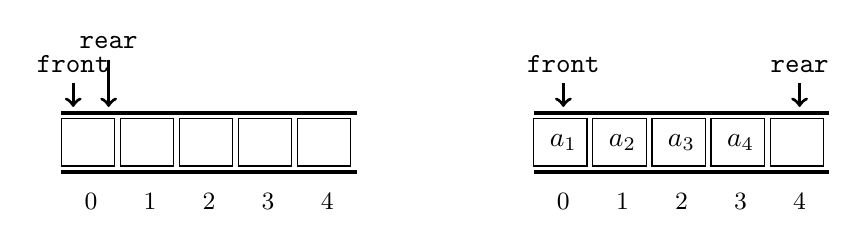
\begin{tikzpicture}
    \tikzstyle{information text}=[rounded corners,fill=blue!10,inner sep=1ex]
    \def\x{0.75}
    \def\y{0.75}

    \foreach \c in {0}{
      \ifthenelse{\c=0}{
        \def\r{0}
        \draw[very thick](\r*\x,\c*\y)--(\r*\x+5*\x,\c*\y);
        \draw[very thick](\r*\x,\c*\y+\y)--(\r*\x+5*\x,\c*\y+\y);        
        \foreach \r in {0,1,2,3,4}{                   
          \node[]at(\r*\x+0.5*\x,\c*\y-0.5*\y){\small $\r$};
        }

        \foreach \r in {1,2,3,4,5}{         
          \draw[](\r*\x-\x,\c*\y+0.1*\y)rectangle(\r*\x-0.1*\x,\c*\y+0.9*\y);
        }

        \def\r{1}
        \draw[->,very thick](\r*\x-0.8*\x,\c*\y+1.5*\y)node[above]{{\tt front}}--(\r*\x-0.8*\x,\c*\y+1.1*\y) ;
        \draw[->,very thick](\r*\x-0.2*\x,\c*\y+1.9*\y)node[above]{{\tt rear}}--(\r*\x-0.2*\x,\c*\y+1.1*\y) ;

        %% \pause
        \def\rr{8}
        %% \draw[very thick,->](\rr*\x-2.8*\x,\c*\y+0.5*\y)--node[above]{出队列}(\rr*\x-0.2*\x,\c*\y+0.5*\y);

        %% \pause
        
        \draw[very thick](\rr*\x,\c*\y)--(\rr*\x+5*\x,\c*\y);
        \draw[very thick](\rr*\x,\c*\y+\y)--(\rr*\x+5*\x,\c*\y+\y);
        \foreach \r in {0,1,2,3,4}{                   
          \node[]at(\r*\x+\rr*\x+0.5*\x,\c*\y-0.5*\y){\small $\r$};
        }

        \def\rr{8}
        \foreach \r in {1,2,3,4,5}{         
          \draw[](\r*\x+\rr*\x-\x,\c*\y+0.1*\y)rectangle(\r*\x+\rr*\x-0.1*\x,\c*\y+0.9*\y);
        }
        \foreach \r in {1,2,3,4}{         
          \node[]at(\r*\x+\rr*\x-0.5*\x,\c*\y+0.5*\y){$a_{\r}$};
        }

        \def\r{1}
        \draw[->,very thick](\r*\x+\rr*\x-0.5*\x,\c*\y+1.5*\y)node[above]{{\tt front}}--(\r*\x+\rr*\x-0.5*\x,\c*\y+1.1*\y) ;
        \def\r{5}
        \draw[->,very thick](\r*\x+\rr*\x-0.5*\x,\c*\y+1.5*\y)node[above]{{\tt rear}}--(\r*\x+\rr*\x-0.5*\x,\c*\y+1.1*\y) ;
      }
    }
  \end{tikzpicture}
\end{figure}
  
\end{frame}
%
\begin{frame}\ft{\subsecname}
\begin{figure}
  \centering
  \begin{tikzpicture}
    \tikzstyle{information text}=[rounded corners,fill=blue!10,inner sep=1ex]
    \def\x{0.75}
    \def\y{0.75}

    \foreach \c in {0}{
      \ifthenelse{\c=0}{
        \def\r{0}
        \def\rr{0}
        \draw[very thick](\r*\x,\c*\y)--(\r*\x+5*\x,\c*\y);
        \draw[very thick](\r*\x,\c*\y+\y)--(\r*\x+5*\x,\c*\y+\y);        
        \foreach \r in {0,1,2,3,4}{                   
          \node[]at(\r*\x+0.5*\x,\c*\y-0.5*\y){\small $\r$};
        }

        \foreach \r in {1,2,3,4,5}{         
          \draw[](\r*\x-\x,\c*\y+0.1*\y)rectangle(\r*\x-0.1*\x,\c*\y+0.9*\y);
        }
        \foreach \r in {3,4}{         
          \node[]at(\r*\x+\rr*\x-0.5*\x,\c*\y+0.5*\y){$a_{\r}$};
        }

        \def\r{3}
        \draw[->,very thick](\r*\x+\rr*\x-0.5*\x,\c*\y+1.5*\y)node[above]{{\tt front}}--(\r*\x+\rr*\x-0.5*\x,\c*\y+1.1*\y) ;
        \def\r{4}
        \draw[->,very thick](\r*\x+\rr*\x-0.5*\x,\c*\y+1.9*\y)node[above]{{\tt rear}}--(\r*\x+\rr*\x-0.5*\x,\c*\y+1.1*\y) ;

        %% \pause
        \def\rr{8}
        %% \draw[very thick,->](\rr*\x-2.8*\x,\c*\y+0.5*\y)--node[above]{出队列}(\rr*\x-0.2*\x,\c*\y+0.5*\y);

        %% \pause
        
        \draw[very thick](\rr*\x,\c*\y)--(\rr*\x+5*\x,\c*\y);
        \draw[very thick](\rr*\x,\c*\y+\y)--(\rr*\x+5*\x,\c*\y+\y);
        \foreach \r in {0,1,2,3,4}{                   
          \node[]at(\r*\x+\rr*\x+0.5*\x,\c*\y-0.5*\y){\small $\r$};
        }

        \def\rr{8}
        \foreach \r in {1,2,3,4,5}{         
          \draw[](\r*\x+\rr*\x-\x,\c*\y+0.1*\y)rectangle(\r*\x+\rr*\x-0.1*\x,\c*\y+0.9*\y);
        }
        \foreach \r in {3,4,5}{         
          \node[]at(\r*\x+\rr*\x-0.5*\x,\c*\y+0.5*\y){$a_{\r}$};
        }

        \def\r{3}
        \draw[->,very thick](\r*\x+\rr*\x-0.5*\x,\c*\y+1.5*\y)node[above]{{\tt front}}--(\r*\x+\rr*\x-0.5*\x,\c*\y+1.1*\y) ;
        \def\r{6}
        \draw[->,very thick](\r*\x+\rr*\x-0.5*\x,\c*\y+1.5*\y)node[above]{{\tt rear}}--(\r*\x+\rr*\x-0.5*\x,\c*\y+1.1*\y) ;

 
        \def\r{6}
        \node[]at(\r*\x+\rr*\x-0.5*\x,\c*\y+0.5*\y){
\includegraphics[width=0.5cm]{Chapters/Ch03/Tikz/question.jpg}};
        
      }
    }
  \end{tikzpicture}
\end{figure}

\pause

\begin{itemize}
\item $a_1, a_2$出队,{\tt front}指向下标为2的位置,{\tt rear}不变;\\[0.1in]
\item 接着$a_5$入队,{\tt front}不变,{\tt rear}移动到数组之外;\\[0.1in]
\item 若接着入队,会产生数组越界的错误。可实际上,前两个位置还空闲,这种现象称为“假溢出”。
\end{itemize}
\end{frame}
%

\begin{frame}\ft{\subsecname}
\begin{dingyi}
头尾相连的队列顺序存储结构称为循环队列。
\end{dingyi}
\end{frame}
%
%
\begin{frame}\ft{\subsecname}
将上图中的{\tt rear}指向下标为0的位置,就不会造成指针指向不明的问题。
\begin{figure}
  \centering
  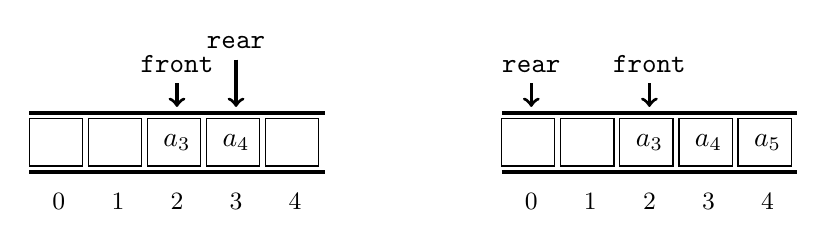
\begin{tikzpicture}
    \tikzstyle{information text}=[rounded corners,fill=blue!10,inner sep=1ex]
    \def\x{0.75}
    \def\y{0.75}

    \foreach \c in {0}{
      \ifthenelse{\c=0}{
        \def\r{0}
        \def\rr{0}
        \draw[very thick](\r*\x,\c*\y)--(\r*\x+5*\x,\c*\y);
        \draw[very thick](\r*\x,\c*\y+\y)--(\r*\x+5*\x,\c*\y+\y);        
        \foreach \r in {0,1,2,3,4}{                   
          \node[]at(\r*\x+0.5*\x,\c*\y-0.5*\y){\small $\r$};
        }

        \foreach \r in {1,2,3,4,5}{         
          \draw[](\r*\x-\x,\c*\y+0.1*\y)rectangle(\r*\x-0.1*\x,\c*\y+0.9*\y);
        }
        \foreach \r in {3,4}{         
          \node[]at(\r*\x+\rr*\x-0.5*\x,\c*\y+0.5*\y){$a_{\r}$};
        }

        \def\r{3}
        \draw[->,very thick](\r*\x+\rr*\x-0.5*\x,\c*\y+1.5*\y)node[above]{{\tt front}}--(\r*\x+\rr*\x-0.5*\x,\c*\y+1.1*\y) ;
        \def\r{4}
        \draw[->,very thick](\r*\x+\rr*\x-0.5*\x,\c*\y+1.9*\y)node[above]{{\tt rear}}--(\r*\x+\rr*\x-0.5*\x,\c*\y+1.1*\y) ;

        %% \pause
        \def\rr{8}
        %% \draw[very thick,->](\rr*\x-2.8*\x,\c*\y+0.5*\y)--node[above]{出队列}(\rr*\x-0.2*\x,\c*\y+0.5*\y);

        %% \pause
        
        \draw[very thick](\rr*\x,\c*\y)--(\rr*\x+5*\x,\c*\y);
        \draw[very thick](\rr*\x,\c*\y+\y)--(\rr*\x+5*\x,\c*\y+\y);
        \foreach \r in {0,1,2,3,4}{                   
          \node[]at(\r*\x+\rr*\x+0.5*\x,\c*\y-0.5*\y){\small $\r$};
        }

        \def\rr{8}
        \foreach \r in {1,2,3,4,5}{         
          \draw[](\r*\x+\rr*\x-\x,\c*\y+0.1*\y)rectangle(\r*\x+\rr*\x-0.1*\x,\c*\y+0.9*\y);
        }
        \foreach \r in {3,4,5}{         
          \node[]at(\r*\x+\rr*\x-0.5*\x,\c*\y+0.5*\y){$a_{\r}$};
        }

        \def\r{3}
        \draw[->,very thick](\r*\x+\rr*\x-0.5*\x,\c*\y+1.5*\y)node[above]{{\tt front}}--(\r*\x+\rr*\x-0.5*\x,\c*\y+1.1*\y) ;
        \def\r{1}
        \draw[->,very thick](\r*\x+\rr*\x-0.5*\x,\c*\y+1.5*\y)node[above]{{\tt rear}}--(\r*\x+\rr*\x-0.5*\x,\c*\y+1.1*\y) ;
        
      }
    }
  \end{tikzpicture}
\end{figure}
  
\end{frame}

\begin{frame}\ft{\subsecname}
\begin{figure}
  \centering
  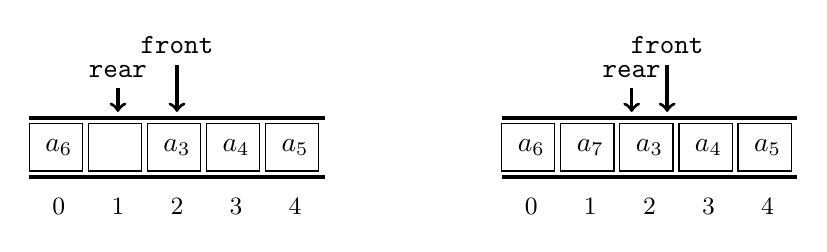
\begin{tikzpicture}
    \tikzstyle{information text}=[rounded corners,fill=blue!10,inner sep=1ex]
    \def\x{0.75}
    \def\y{0.75}

    \foreach \c in {0}{
      \ifthenelse{\c=0}{
        \def\r{0}
        \def\rr{0}
        \draw[very thick](\r*\x+\rr*\x,\c*\y)--(\r*\x+\rr*\x+5*\x,\c*\y);
        \draw[very thick](\r*\x+\rr*\x,\c*\y+\y)--(\r*\x+\rr*\x+5*\x,\c*\y+\y);        
        \foreach \r in {0,1,2,3,4}{                   
          \node[]at(\r*\x+\rr*\x+0.5*\x,\c*\y-0.5*\y){\small $\r$};
        }

        \foreach \r in {1,2,3,4,5}{         
          \draw[](\r*\x+\rr*\x-\x,\c*\y+0.1*\y)rectangle(\r*\x+\rr*\x-0.1*\x,\c*\y+0.9*\y);
        }
        \foreach \r in {3,4,5}{         
          \node[]at(\r*\x+\rr*\x-0.5*\x,\c*\y+0.5*\y){$a_{\r}$};
        }
        \def\r{3}
        \draw[->,very thick](\r*\x+\rr*\x-0.5*\x,\c*\y+1.9*\y)node[above]{{\tt front}}--(\r*\x+\rr*\x-0.5*\x,\c*\y+1.1*\y) ;
        \def\r{2}
        \draw[->,very thick](\r*\x+\rr*\x-0.5*\x,\c*\y+1.5*\y)node[above]{{\tt rear}}--(\r*\x+\rr*\x-0.5*\x,\c*\y+1.1*\y) ;
        \def\r{1}
        \def\rrr{6}
        \node[]at(\r*\x+\rr*\x-0.5*\x,\c*\y+0.5*\y){$a_{\rrr}$};

        %% %% %% %% %% %% %% 
        \def\rr{8}
        \draw[very thick](\rr*\x,\c*\y)--(\rr*\x+5*\x,\c*\y);
        \draw[very thick](\rr*\x,\c*\y+\y)--(\rr*\x+5*\x,\c*\y+\y);
        \foreach \r in {0,1,2,3,4}{                   
          \node[]at(\r*\x+\rr*\x+0.5*\x,\c*\y-0.5*\y){\small $\r$};
        }

        \def\rr{8}
        \foreach \r in {1,2,3,4,5}{         
          \draw[](\r*\x+\rr*\x-\x,\c*\y+0.1*\y)rectangle(\r*\x+\rr*\x-0.1*\x,\c*\y+0.9*\y);
        }
        \foreach \r in {3,4,5}{         
          \node[]at(\r*\x+\rr*\x-0.5*\x,\c*\y+0.5*\y){$a_{\r}$};
        }

        \def\r{3}
        \draw[->,very thick](\r*\x+\rr*\x-0.8*\x,\c*\y+1.5*\y)node[above]{{\tt rear}}--(\r*\x+\rr*\x-0.8*\x,\c*\y+1.1*\y) ;
        \draw[->,very thick](\r*\x+\rr*\x-0.2*\x,\c*\y+1.9*\y)node[above]{{\tt front}}--(\r*\x+\rr*\x-0.2*\x,\c*\y+1.1*\y) ;
        \def\r{1}
        \def\rrr{6}
        \node[]at(\r*\x+\rr*\x-0.5*\x,\c*\y+0.5*\y){$a_{\rrr}$};
        \def\r{2}
        \def\rrr{7}
        \node[]at(\r*\x+\rr*\x-0.5*\x,\c*\y+0.5*\y){$a_{\rrr}$};
        
      }
    }
  \end{tikzpicture}
\end{figure}

\pause

\begin{itemize}
\item 接着$a_6$入队,放置于下标为0处,而{\tt rear}指向下标为1处。\\[0.1in]
\item 再让$a_7$入队,则{\tt rear}与{\tt front}重合。
\end{itemize}

\end{frame}

\begin{frame}\ft{\subsecname}
\begin{wenti}
空队列时,{\tt front==rear},现在队列已满,仍然有{\tt front==rear},如何判断队列是空是满?
\end{wenti}
\pause 
\begin{itemize}
\item[(1)] 设置一个标志变量{\tt flag},当{\tt front == rear \&\& flag == 0}时队列为空;
而当{\tt front == rear \&\& flag==1}时队列为满。\\[0.1in]
\pause 
\item[(2)] 当队列为空时,条件就为{\tt front == rear};当队列满时,修改其条件,让数组中始终保留一个空闲单元。
\end{itemize}
\end{frame}

\begin{frame}\ft{\subsecname}
\begin{figure}
  \centering
  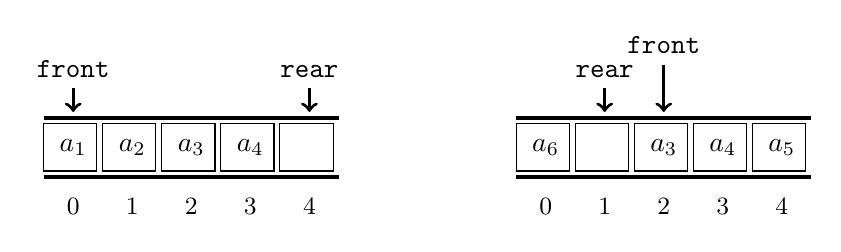
\begin{tikzpicture}
    \tikzstyle{information text}=[rounded corners,fill=blue!10,inner sep=1ex]
    \def\x{0.75}
    \def\y{0.75}

    \foreach \c in {0}{
      \ifthenelse{\c=0}{
        \def\r{0}
        \def\rr{0}
        \draw[very thick](\r*\x+\rr*\x,\c*\y)--(\r*\x+\rr*\x+5*\x,\c*\y);
        \draw[very thick](\r*\x+\rr*\x,\c*\y+\y)--(\r*\x+\rr*\x+5*\x,\c*\y+\y);        
        \foreach \r in {0,1,2,3,4}{                   
          \node[]at(\r*\x+\rr*\x+0.5*\x,\c*\y-0.5*\y){\small $\r$};
        }

        \foreach \r in {1,2,3,4,5}{         
          \draw[](\r*\x+\rr*\x-\x,\c*\y+0.1*\y)rectangle(\r*\x+\rr*\x-0.1*\x,\c*\y+0.9*\y);
        }
        \foreach \r in {1,2,3,4}{         
          \node[]at(\r*\x+\rr*\x-0.5*\x,\c*\y+0.5*\y){$a_{\r}$};
        }
        \def\r{1}
        \draw[->,very thick](\r*\x+\rr*\x-0.5*\x,\c*\y+1.5*\y)node[above]{{\tt front}}--(\r*\x+\rr*\x-0.5*\x,\c*\y+1.1*\y) ;
        \def\r{5}
        \draw[->,very thick](\r*\x+\rr*\x-0.5*\x,\c*\y+1.5*\y)node[above]{{\tt rear}}--(\r*\x+\rr*\x-0.5*\x,\c*\y+1.1*\y) ;

        %%%%%%%%%%%%%%%% 
        \def\rr{8}
        \draw[very thick](\rr*\x,\c*\y)--(\rr*\x+5*\x,\c*\y);
        \draw[very thick](\rr*\x,\c*\y+\y)--(\rr*\x+5*\x,\c*\y+\y);
        \foreach \r in {0,1,2,3,4}{                   
          \node[]at(\r*\x+\rr*\x+0.5*\x,\c*\y-0.5*\y){\small $\r$};
        }

        \def\rr{8}
        \foreach \r in {1,2,3,4,5}{         
          \draw[](\r*\x+\rr*\x-\x,\c*\y+0.1*\y)rectangle(\r*\x+\rr*\x-0.1*\x,\c*\y+0.9*\y);
        }
        \foreach \r in {3,4,5}{         
          \node[]at(\r*\x+\rr*\x-0.5*\x,\c*\y+0.5*\y){$a_{\r}$};
        }

        \def\r{3}
        \draw[->,very thick](\r*\x+\rr*\x-0.5*\x,\c*\y+1.9*\y)node[above]{{\tt front}}--(\r*\x+\rr*\x-0.5*\x,\c*\y+1.1*\y) ;
        \def\r{2}
        \draw[->,very thick](\r*\x+\rr*\x-0.5*\x,\c*\y+1.5*\y)node[above]{{\tt rear}}--(\r*\x+\rr*\x-0.5*\x,\c*\y+1.1*\y) ;
        \def\r{1}
        \def\rrr{6}
        \node[]at(\r*\x+\rr*\x-0.5*\x,\c*\y+0.5*\y){$a_{\rrr}$};
        
      }
    }
  \end{tikzpicture}
\end{figure}
  
\end{frame}

\begin{frame}[fragile]\ft{\subsecname}
\begin{wenti}
对于第二种办法,由于{\tt rear}可能比{\tt front}大,也可能比{\tt front}小,如何判定队列是否为满?
\end{wenti}
\vspace{0.1in}\pause 

设队列的最大尺寸为{\tt MAXSIZE},则队列满的条件是

{\tt (rear + 1) \% MAXSIZE == front}

\end{frame}

\begin{frame}[fragile]\ft{\subsecname}
\begin{wenti}
如何计算队列的长度?
\end{wenti}
\vspace{0.1in}\pause 

当{\tt rear > front}时,队列长度为{\tt rear - front};  \vspace{0.1in}\pause

当{\tt rear < front}时,队列长度分为两段,一段为{\tt MAXSIZE - front},另一段为{\tt rear - 0},合计为{\tt rear - front + MAXSIZE}。  \vspace{0.1in}\pause

故通用的队列长度计算公式为

{\tt  (rear - front + MAXSIZE) / MAXSIZE}
\end{frame}


\begin{frame}\ft{\subsecname}

\textcolor{acolor5}{\Large 循环队列之完整程序}

\end{frame}


\begin{frame}\ft{{\tt SqQueue.h}}
\lstinputlisting[
language=C,
]{Chapters/Ch03/Code/SqQueue/SqQueue.h}
\end{frame}


\begin{frame}\ft{{\tt Init.c}}
\lstinputlisting[
language=C,
]{Chapters/Ch03/Code/SqQueue/Init.c}
\end{frame}

\begin{frame}\ft{\tt Length.c}
\lstinputlisting[
language=C,
]{Chapters/Ch03/Code/SqQueue/Length.c}
\end{frame}

\begin{frame}\ft{\tt Enter.c}
\lstinputlisting[
language=C,
]{Chapters/Ch03/Code/SqQueue/Enter.c}
\end{frame}

\begin{frame}\ft{\tt Exit.c}
\lstinputlisting[
language=C,
]{Chapters/Ch03/Code/SqQueue/Exit.c}
\end{frame}
